\section{Comparing Sizes}

\subsection{The Beginning}

Let's suppose I have two collections of things: for example, students and chairs.\footnote{This example comes from a class I took in the spring of 2019, ``MATH 432: Set Theory and Topology'' at the University of Illinois at Urbana-Champaign, taught by Anush Tserunyan.}
I want to answer the question, ``Are there more students, or more chairs?''
This is quite a reasonable question to ask: maybe I need to get more chairs to accomodate all the students, or perhaps there can be more students in this class because we have so many extra chairs.

Answering the question is not too difficult in a typical classroom: I need only count the number of students and the number of chairs, then see which is larger.
However, there is another way, which takes much less effort on my part: tell the students to each sit down in a chair.
After they're done, I can tell whether there are more students or more chairs easily: if there are students standing, because there are not enough chairs, then there are more students than chairs; otherwise, if there are empty chairs, and no standing students, then there are more chairs; if there are neither standing students nor empty chairs, there are exactly the same amount of students and chairs.
This approach also scales better: if I am in a huge lecture hall that can hold 600 students, it would take a long time to count each student and each chair, but I can let the students sit down and easily have my answer.

This approach gives me an \emph{assignment} of students to chairs: that is, if I label each student (e.g., from $1$ to $n$) and each chair with a number (e.g., from $1$ to $m$), then every student $i$ gets assigned to some chair $j$.
The assignment is the list of these pairs, for example, if I have students labeled $1,2,3,4$ and chairs labeled $1,2,3,4$, then an assignment might be $(1,1)$, $(2,2)$, $(3,3)$ and $(4,4)$.
I didn't put any condition on the assignments, except that it must pick one chair for every student.
However, the following is also an assignment: $(1,1)$, $(2,1)$, $(3,1)$, $(4,1)$; that is, the assignment in which each student gets assigned the same chair.
Clearly, this is a ``bad'' assignment.
So what are the conditions for being a ``good'' assignment?
\reed{Have them think about this?}

A \emph{good} assignment is one that doesn't assign the same chair to two different students.
Put another way, if student $a$ and student $b$ are assigned to the same chair $j$, then $a = b$. \reed{Is this important?}

So now we can make a statement about assignments: if we can create a good assignment, then there cannot be more students than chairs, and vice versa.
Why is this true?
Well, if we can create a good assignment, then each student gets their own chair, meaning we must have at least one chair per student.
Of course, there could be chairs left over, but there must be at least one per student.

For the vice versa part, if there are no more students then chairs, then we can build an assignment as follows.
Start out with no students assigned to a chair.
Pick any student $i_1$, and any chair $j_1$; remember that we don't know how the students and chairs are labeled, just that they are labeled in some way, so we can't say ``pick student 1''.
For example, they might be labeled by name, rather than number.
You can think of what we're doing as ``relabeling'' the students with numbers.
Add $(i_1,j_1)$ to the assignment.
Then pick a student other than $i$ and a chair other than $j$, if there are any students left to assign (this could be a very small class with just one student).
If there is such a student $i_2$, there must be some chair $j_2$ other than $j$, or there would be more students than chairs, which we assumed wasn't the case.
Then add $(i_2, j_2)$ to the assignment.
Again, if there are any students not yet assigned to a chair, pick a student $i_3$ and a chair $j_3$ that have not yet been assigned: there must be some chair because otherwise there would be more students than chairs.
Add $(i_3, j_3)$ to the assignment.
I hope you will believe we when I say we can repeat this argument as many times as required to assign every student to a chair that has not been chosen before.

So then our statement ``if we can create a good assignment, then there cannot be more students than chairs, and vice versa'' is true.

Let's say that an assignment is \emph{complete} if every chair has a student assigned to it.
Then we can say that if there is a complete assignment, then there are no more chairs than students, and vice versa.

From now on, we'll state this sort of thing as ``there is a complete assignment if and only if there are no more chairs than students.''
This means that, if there is a complete assignment, then there are no more chairs than students, and, if there are no more chairs than students, then there is a complete assignment.
So this statement is a sort of \emph{compound} statement: there are multiple parts to it.
In order to prove it, we need to prove every part of the statement.

From now on, we will write claims like the above as \emph{theorems}, \emph{propositions}, and \emph{lemmas}, generally in decreasing order of importance.
\reed{Go through and convert all the propositions after this too}

So we'll write the above claims as:
\begin{theorem}
    There is a complete assignment if and only if there are no more chairs than students.
\end{theorem}

Every claim must be proven, so theorems, propositions, and lemmas will be accompanied by a proof, like the following.
The square at the end of the proof indicates that the proof is complete.

\begin{proof}
    Let's start with the first part: if there is a complete assignment, then there are no more chairs than students.
    If there is a complete assignment, then every chair has some student assignment to it, by definition.
    So take the students that we assigned to chairs out of our list of students.
    Either the list is empty, so there are exactly as many students as chairs, or the list is not empty, and there are more students than chairs.
    In either case, there are at least as many students as chairs: or, put another way, there are no more chairs than students.

    And now let's do the second part: if there are no more chairs than students, then there is a complete assignment.
    That is, we want to build a complete assignment.
    We'll do this similarly to how we built the good assignment for our previous statement.
    Let's start with no students assigned to no chairs.
    If there's no chairs at all, then we're done.
    Otherwise, let's pick one of the remaining chairs: $j_1$.
    Because there are at least as many students as chairs, there has to be at least one student, so let's pick any random student $i_1$ to assign to $j_1$.
    As we did before, we simply repeat this process to build the assignment.
    At each stage, if we have chairs left to assign, we must also have students left to assign, because we remove one chair and one student from each list for each assignment, meaning that if we had at least as many students as chairs before making a choice, then we must also have at least as many students as chairs afterwards.
\end{proof}

So we now know two things for sure: if we have a good assignment, then there are at least as many chairs as students; and if we have a complete assignment, then there are at least as many students as chairs.
We also know the converses \reed{define converse at some point} hold, but let's just put that aside for now.
What if we have an assignment that is both good \textbf{and} complete?
Then we have at least as many chairs as students, and at least as many students as chairs: that means we have the same amount of students and chairs.
We'll write this as $\samenumber{S}{C}$, where $S$ is all the students and $C$ is all the chairs.

This is an example of mathematical reasoning.
\reed{talk more about this part, summarizing}

\subsection{Onto Infinity}

\reed{For the beginning, keep things vague. Hopefully strange results will make it naturally clear why we need to be more rigorous and specific}

What if we talk about assigning things other than students and chairs?

For example, what I want to assign apples to people, or names to people, or addresses to buildings?
Obviously there are many, many examples of assignments.
And our arguments from the previous section are still valid for these other kinds of assignments!

For example, let's consider a good assignment of apples to people: that would mean that the same apple isn't assigned to two different people.
If we have a good assignment of apples to people, meaning that no two different people are assigned same apple.
In that case, it's perhaps quite clear that there are at least as many people as apples\footnote{Assuming we must assign every apple to someone: we don't want them to go to waste!}: if not, we can use the same argument from above to prove this.
Similarly, a complete assignment of apples to people, meaning that every person is assign an apple, or that we have enough apples for everyone.
Then again, if we have a good, complete assignment of apples to people, then we have the same amount of apples as people.

What if we extend this idea even further?
Going back to our students and chairs, what if we had infinitely many students and chairs?
For example, if we have one student and one chair for each \reed{What to call positive integers?} positive integer: that is, for every positive integer $i$, we have some student $\text{Student}_i$ and some chair $\text{Chair}_i$.
Before, when we had a good, complete assignment of students to chairs, we knew that we have the same amount of students and chairs.
In this case, because we have one student and one chair for each positive integer, it seems natural to say we have as many students as chairs, even if we wouldn't say we have the same \textbf{number} of students and chairs.
We still have a good, complete assignment of students to chairs: assign $\text{Student}_i$ to $\text{Chair}_i$.
For the rest of this chapter we'll refer to $\text{Student}_i$ as $s_i$ and $\text{Chair}_i$ as $c_i$.

Now suppose that, one day, as this infinite class is working on some lesson, a new student, who we'll just call $s_0$, comes to the class.
It seems we have a problem: where will they sit?
How can we make space for them?
\reed{Have them think about it for a while}

In fact, the answer isn't too complicated, just a little tricky to come up with: tell each student to ``move over'' one seat.
What does this mean exactly?
Well, before, we assigned student $s_i$ to chair $c_i$.
Now we assign student $s_i$ to seat $c_{i+1}$.
Then the first chair, $c_1$ is free, so assign the new student $s_0$ to chair $c_1$.
The diagram below shows this assignment.

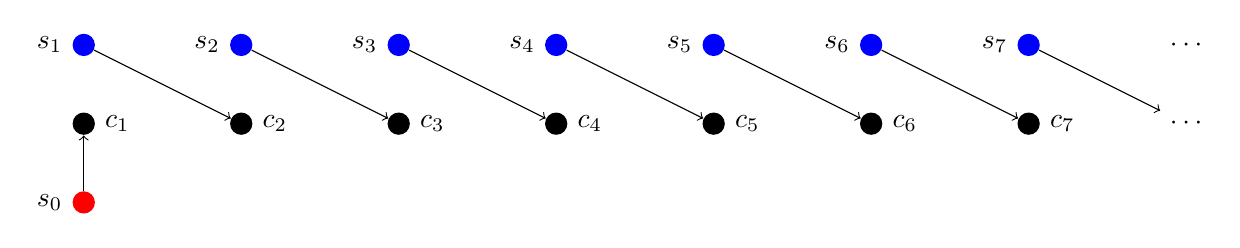
\begin{tikzpicture}
    \node[circle, fill=blue, inner sep=0.1cm, label=left:$s_1$] (s1) at (0, 1) {};
    \node[circle, fill=blue, inner sep=0.1cm, label=left:$s_2$] (s2) at (2, 1) {};
    \node[circle, fill=blue, inner sep=0.1cm, label=left:$s_3$] (s3) at (4, 1) {};
    \node[circle, fill=blue, inner sep=0.1cm, label=left:$s_4$] (s4) at (6, 1) {};
    \node[circle, fill=blue, inner sep=0.1cm, label=left:$s_5$] (s5) at (8, 1) {};
    \node[circle, fill=blue, inner sep=0.1cm, label=left:$s_6$] (s6) at (10, 1) {};
    \node[circle, fill=blue, inner sep=0.1cm, label=left:$s_7$] (s7) at (12, 1) {};
    \node[] (srest) at (14, 1) {$\cdots$};

    \node[circle, fill=black, inner sep=0.1cm, label=right:$c_1$] (c1) at (0, 0) {};
    \node[circle, fill=black, inner sep=0.1cm, label=right:$c_2$] (c2) at (2, 0) {};
    \node[circle, fill=black, inner sep=0.1cm, label=right:$c_3$] (c3) at (4, 0) {};
    \node[circle, fill=black, inner sep=0.1cm, label=right:$c_4$] (c4) at (6, 0) {};
    \node[circle, fill=black, inner sep=0.1cm, label=right:$c_5$] (c5) at (8, 0) {};
    \node[circle, fill=black, inner sep=0.1cm, label=right:$c_6$] (c6) at (10, 0) {};
    \node[circle, fill=black, inner sep=0.1cm, label=right:$c_7$] (c7) at (12, 0) {};
    \node[] (crest) at (14, 0) {$\cdots$};

    \node[circle, fill=red, inner sep=0.1cm, label=left:$s_0$] (s1n) at (0, -1) {};

    \draw[->] (s1) -- (c2);
    \draw[->] (s2) -- (c3);
    \draw[->] (s3) -- (c4);
    \draw[->] (s4) -- (c5);
    \draw[->] (s5) -- (c6);
    \draw[->] (s6) -- (c7);
    \draw[->] (s7) -- (crest);

    \draw[->] (s1n) -- (c1);
\end{tikzpicture}

Now every student is assigned to a chair, and every chair has a student. \reed{More explanation is probably need: clarify this is a good and complete assignment}
So then we \textbf{still} have as many chairs as students!
So adding one new student poses no issues: in fact, this also means that we can add two, three, four, etc. students.
How?
Just move everyone over one seat, then over again, etc.
\reed{This previous sentence should probably be an exercise}?
We could also say ``move everyone over two/three/four seats'', but then we have to define the assignment again; if we say move over one seat, then move over one more, we've achieved the same thing, but there's no need to prove that this works because we already have.
\reed{This previous sentence is only sort of true: we basically proved we can add one thing to natural numbers, but not that we can do it again...}

\paragraph{Adding Infinitely Many Students}
Intuitively, perhaps it makes sense that we can add any finite number of students to our class, because our class is so big that a finite addition basically makes no difference in the number of students.
But what if we want to add \textbf{infinitely more} students? For example, suppose we want to double the size of our class.
Specically, for every student $s_i$, we add a second student $s_{i}'$, but we don't add any more chairs.
Do we still have enough chairs for everyone?

At first glance, you might, quite reasonably, think there is no way that we could possibly have enough chairs for twice as many people.
We can't use our old strategy of just moving people over one at a time until we have enough seats, because we have to move over infinitely many times: we'll never finish!
It's very important that we be able to write down a complete description of our assignment; otherwise, how could anyone read it to tell what seat they should be in?
I don't mean that we have to list out the whole assignment, only that we have some finite way to describe the assignment; just enough to answer the question ``where should I sit?''
For example, if student 10, $s_{10}$ asks where they should sit, we can easily look at the (previous) assignment we gave, and say ``chair $c_{11}$.''
So if we can't use our old strategy, can we do it any other way, or is it impossible?

By impossible, I don't mean \textbf{really hard}, or ``I can't think of how to do it'', I mean, actually, provably, impossible.
For example, I can prove that you can't have a good assignment if you have $2$ students and only $1$ chair, or if you have infinitely many students, and finitely many chairs. \reed{Should we actually write out these proofs}

In fact, it is possible to assign each student in this new, larger class, to a chair; specfically, I claim there is a good, complete assignment.
Instead of telling everyone to move over one seat, we tell the first student to move over one chair, the second student to move over three, the third student to move over five, and so on.
Then the first new student sits in the first chair, the second new student sits in the third chair, the third new student sits in the fifth chair, and so on.
The diagram below shows this assignment:

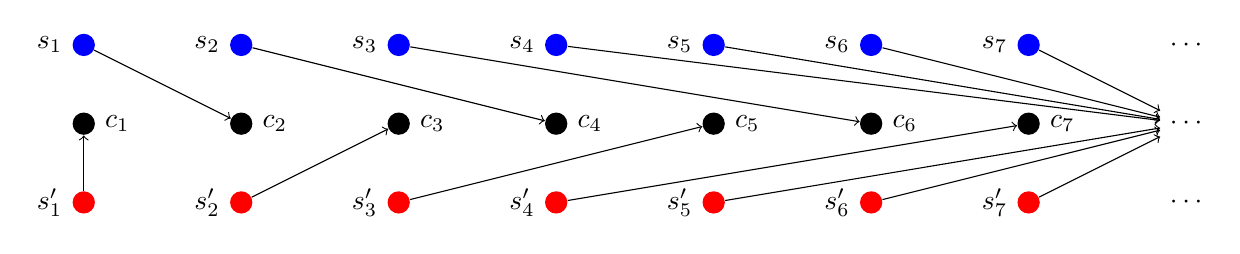
\begin{tikzpicture}
    \node[circle, fill=blue, inner sep=0.1cm, label=left:$s_1$] (s1) at (0, 1) {};
    \node[circle, fill=blue, inner sep=0.1cm, label=left:$s_2$] (s2) at (2, 1) {};
    \node[circle, fill=blue, inner sep=0.1cm, label=left:$s_3$] (s3) at (4, 1) {};
    \node[circle, fill=blue, inner sep=0.1cm, label=left:$s_4$] (s4) at (6, 1) {};
    \node[circle, fill=blue, inner sep=0.1cm, label=left:$s_5$] (s5) at (8, 1) {};
    \node[circle, fill=blue, inner sep=0.1cm, label=left:$s_6$] (s6) at (10, 1) {};
    \node[circle, fill=blue, inner sep=0.1cm, label=left:$s_7$] (s7) at (12, 1) {};
    \node[] (srest) at (14, 1) {$\cdots$};

    \node[circle, fill=black, inner sep=0.1cm, label=right:$c_1$] (c1) at (0, 0) {};
    \node[circle, fill=black, inner sep=0.1cm, label=right:$c_2$] (c2) at (2, 0) {};
    \node[circle, fill=black, inner sep=0.1cm, label=right:$c_3$] (c3) at (4, 0) {};
    \node[circle, fill=black, inner sep=0.1cm, label=right:$c_4$] (c4) at (6, 0) {};
    \node[circle, fill=black, inner sep=0.1cm, label=right:$c_5$] (c5) at (8, 0) {};
    \node[circle, fill=black, inner sep=0.1cm, label=right:$c_6$] (c6) at (10, 0) {};
    \node[circle, fill=black, inner sep=0.1cm, label=right:$c_7$] (c7) at (12, 0) {};
    \node[] (crest) at (14, 0) {$\cdots$};

    \node[circle, fill=red, inner sep=0.1cm, label=left:$s_1'$] (s1n) at (0, -1) {};
    \node[circle, fill=red, inner sep=0.1cm, label=left:$s_2'$] (s2n) at (2, -1) {};
    \node[circle, fill=red, inner sep=0.1cm, label=left:$s_3'$] (s3n) at (4, -1) {};
    \node[circle, fill=red, inner sep=0.1cm, label=left:$s_4'$] (s4n) at (6, -1) {};
    \node[circle, fill=red, inner sep=0.1cm, label=left:$s_5'$] (s5n) at (8, -1) {};
    \node[circle, fill=red, inner sep=0.1cm, label=left:$s_6'$] (s6n) at (10, -1) {};
    \node[circle, fill=red, inner sep=0.1cm, label=left:$s_7'$] (s7n) at (12, -1) {};
    \node[] (snrest) at (14, -1) {$\cdots$};

    \draw[->] (s1) -- (c2);
    \draw[->] (s2) -- (c4);
    \draw[->] (s3) -- (c6);
    \draw[->] (s4) -- (crest);
    \draw[->] (s5) -- (crest);
    \draw[->] (s6) -- (crest);
    \draw[->] (s7) -- (crest);

    \draw[->] (s1n) -- (c1);
    \draw[->] (s2n) -- (c3);
    \draw[->] (s3n) -- (c5);
    \draw[->] (s4n) -- (c7);
    \draw[->] (s5n) -- (crest);
    \draw[->] (s6n) -- (crest);
    \draw[->] (s7n) -- (crest);
\end{tikzpicture}

We can write this assignment as follows: assign student $s_i$ to chair $c_{2i+1}$, and student $s_i'$ to chair $c_{2i}$.
Hopefully it is clear from the diagram that each chair will only get one student, and that we will not ``run out'' of chairs to assign students to.
Furthermore, we won't ``miss'' any chairs: every chair gets a student.

So, perhaps surprisingly, there are as many students in our new, doubled class, as in our original class.
Remember, we agreed that if we have a good, complete assignment between a group of students and a group of chairs, then we have the same amount of students and chairs.
We have a good, complete assignment in our original class, and we have a good, complete assignment in our new, doubled class.
So if we have the same amount of students in the original class as chairs, and we have the same amount of students in the new class as we have chairs, then the amount of students in the original class must be the same as the amount of students in the new class.
To write this more concisely, denote the original class of students by $S$, the new class as $S'$, and the chairs by $C$.
Then what I'm saying is: because $\samenumber{S}{C}$ and $\samenumber{S'}{C}$, we can conclude that $\samenumber{S}{S'}$.

If you accept the above \reed{What to do if they don't?}, then we've discovered something somewhat strange.
Let's see how many students we can add to this class.
Essentially, what we did in the previous example is give each student a buddy, so there is a pairing of students, i.e., $s_i$ is ``paired with'' $s_i'$.
What if we gave each student $s_i$ two ``buddies'', $s_i'$ and $s_i''$?
Then we could do the assignment trick above once with $s_i$ and $s_i'$, then again with the new student paired with $c_i$ and $s_i''$ \reed{Clarify this sentence}.
As you can see, we can give each student in the original class any finite number of ``buddies'' (let's call this a group), and we can still find seats for everyone.
We just seat each group together, then move the following groups down by a corresponding amount.

So we can add a ``lot'' of students.
What if give each student infinitely many ``buddies''?
Specifically, for each student $s_i$, there are students $s_{i,1}$, $s_{i,2}$, $s_{i,3}$, and so on for every \reed{positive integer} $j$, there is a student $s_{i,j}$.
Surely that would be too many students?
We definitely can't use our old strategy of seating each group together, because then after the first ``group'', the second group would have to be infinitely far over!
So we're going to have to intersperse the students among each other.
\reed{Have them think about it?}

Again, perhaps very suprisingly, we still have enough chairs!
Consider the following picture, where each row represents one ``group'':

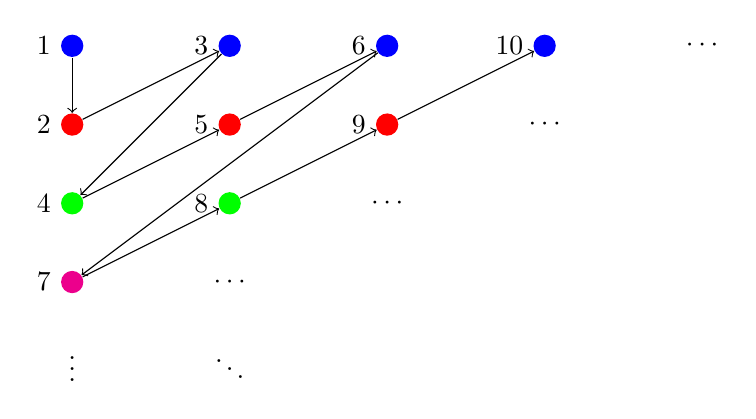
\begin{tikzpicture}
    \node[circle, fill=blue, inner sep=0.1cm, label=left:$1$] (s11) at (0, -1) {};
    \node[circle, fill=blue, inner sep=0.1cm, label=left:$3$] (s21) at (2, -1) {};
    \node[circle, fill=blue, inner sep=0.1cm, label=left:$6$] (s31) at (4, -1) {};
    \node[circle, fill=blue, inner sep=0.1cm, label=left:$10$] (s41) at (6, -1) {};
    \node[] (srest) at (8, -1) {$\cdots$};

    \node[circle, fill=red, inner sep=0.1cm, label=left:$2$] (s12) at (0, -2) {};
    \node[circle, fill=red, inner sep=0.1cm, label=left:$5$] (s22) at (2, -2) {};
    \node[circle, fill=red, inner sep=0.1cm, label=left:$9$] (s32) at (4, -2) {};
    \node[] (srest) at (6, -2) {$\cdots$};

    \node[circle, fill=green, inner sep=0.1cm, label=left:$4$] (s13) at (0, -3) {};
    \node[circle, fill=green, inner sep=0.1cm, label=left:$8$] (s23) at (2, -3) {};
    \node[] (srest) at (4, -3) {$\cdots$};

    \node[circle, fill=magenta, inner sep=0.1cm, label=left:$7$] (s14) at (0, -4) {};
    \node[] (srest) at (2, -4) {$\cdots$};

    \node[] (s1) at (0, -5) {$\vdots$};
    \node[] (s2) at (2, -5) {$\ddots$};

    \draw[->] (s11) edge (s12)
              (s12) edge (s21)
              (s21) edge (s13)
              (s13) edge (s22)
              (s22) edge (s31)
              (s31) edge (s14)
              (s14) edge (s23)
              (s23) edge (s32)
              (s32) edge (s41);
\end{tikzpicture}

We can assign the students by starting at the top left corner, and moving along the grid diagonally, as shown below.
That is, $s_{1,1}$ is assigned to seat $1$, $s_{1,2}$ is assigned to seat $2$, $s_{2,1}$ is assigned to seat $3$, and so on.
Again, we can see that if we go far enough with this process of counting along the diagonal, we can get every student.
That is, we have a good, complete assignment from our new ``infinite buddy'' class to our original group of chairs.
So we must have the same amount of students in the original class as in our new class!

And, of course, this argument extends even further.
If we give each student an infinite number of buddies, and give each of those students an infinite number of friends, and give each of those friends an infinite number of friends, and so on for any finite number of repetitions, we can repeatedly apply the argument above to build a good, complete assignment of students to chairs.

\paragraph{Is it possible to have too many students?}

So even if we add infinitely many students for each student in the original class, we still have the same amount of students!
That's pretty weird, and naturally leads to the following question:

\begin{quote}
    Is it possible to have an amount of students bigger than the original, infinite class?
\end{quote}

After all, infinity is infinity.
What's bigger than infinity?
Must be nothing, of course.
\reed{Maybe we should discuss this a little earlier, to motivate why we even care to show that different sizes of infinity are actually hte ``same''.
I assumed that people \textbf{would} be on board with there being different sizes of infinity, but maybe that's not really the case, and people actually have the opposite view.}

Let's try one more thought experiment, another new way of making a bigger class.
\reed{This analogy maybe needs some work}
Let suppose we add one student for \emph{group of students} in the original class.
For the sake of the experiment, let's say that each new student is assigned exactly one group of student in the original class, who will introduce them to the class and help them with things they're not familiar with.
That is, we have a good, complete assignment from the new students to groups of students in the original class.
We'll write $g$ for a group of students in the original class.
For example, $g$ could be $\curlys{s_1, s_2, s_3, s_4, s_5}$, where the brackets just indicate a group of students, and we'll have some corresponding new student $n_g$, indicating that $n_g$ is assigned to the students 1, 2, 3, 4, and 5.
We could also have some other group $h$ which is $\curlys{s_1, s_3, s_5, s_7, \ldots}$, in other words, all the odd-numbered students.

At first glance, this might seem similar to the previous example, where we give each student an infinite number of buddies, but this is slightly different because we're adding a new student for each group of students in the original class, rather than adding infinitely many students for each student in the original class.
Importantly, we're adding a new student even for the \textbf{infinite} groups of students in the original class rather than just finite groups: this is really what differentiates it from the previous example.
Is it possible that we still have the same number of students even after adding all these students?
Let's even imagine that we make each student in the original class give up their seats, so we're only trying to seat the new students.

In fact, it is not possible to even seat just the new students!
Let's see why: suppose that we did have some good, compelte assignment of the new students to chairs.
That is, each new student $n_g$ is assigned to some chair $c_i$; equivalently, some chair $c_i$ has some new student $n_{g_i}$.
Consider the group of students $m$, where student $s_i$ is in the group $m$ if $s_i$ is \textbf{not} in the group $g_i$.
Let's do the first few together.
Note that below we just pick whether the student is in the group or not arbitrarily, it makes no difference; you can choose any way you want and the argument will still work.
\reed{Is this the best way to explain this?}

\begin{enumerate}
    \item Suppose that student $s_1$ is \textbf{not} in the group $g_1$; then $s_1$ \textbf{is} in the group $m$.
    \item Suppose that student $s_2$ is \textbf{not} in the group $g_2$; then $s_2$ \textbf{is} in the group $m$.
    \item Suppose that student $s_3$ \textbf{is} in the group $g_3$; then $s_3$ is \textbf{not} in the group $m$.
    \item Suppose that student $s_4$ is \textbf{not} in the group $g_4$; then $s_4$ \textbf{is} in the group $m$.
    \item Suppose that student $s_5$ \textbf{is} in the group $g_5$; then $s_5$ is \textbf{not} in the group $m$.
    \item Suppose that student $s_6$ \textbf{is} in the group $g_6$; then $s_6$ is \textbf{not} in the group $m$.
    \item And so on
\end{enumerate}

So in this example, $m$ starts out $\curlys{s_1, s_2, s_4, \ldots}$.
We have a new student for \textbf{every} group of students, so we have a new student for the group $m$, who we called $n_m$.
So what chair is student $n_m$ sitting in?
Well it can't be the first chair: that student doesn't have $s_1$ in their group, but $n_m$ does.
Because their groups aren't the same, they can't be the same student, because each new student has a unique group of students assigned to them.
It can't be second chair: that student doesn't have $s_2$ in their group, but $n_m$ does.
It can't be third chair: that student does have $s_2$ in their group, but $n_m$ doesn't.

In fact, it can't be any chair at all!
Suppose that $n_m$ is sitting in chair $c_i$.
We know that the student sitting there is $n_{g_i}$, so student $n_m$ must be student $n_m$.
But if $n_{g_i}$ has student $s_i$ from the original class in their group, then $n_m$ doesn't have $s_i$ in their group, just by the way we picked the group $m$.
Similarly, if $n_{g_i}$ doesn't have student $s_i$ in their group, then $n_m$ must have $s_i$ in their group!
So their groups don't match, and so the students aren't the same!

Then there has to be at least one student, $n_m$, who doesn't have a chair.
So this isn't a complete, good assignment: in particular, it's not complete.
That means there's no way that we can build a good, complete assignment for all of these new students: there's too many students to seat!
So there are more new students than there were in the original class, because we could seat all the students in the original class.

There's definitely infinite many new students, and infinitely many students in the original class; but there's more new students than students in the original class.
So that means there \textbf{are} ``bigger'' infinities: not all infinite groups are the same size!

\paragraph{What are the properties of ``same amount''?}
\reed{Maybe an interesting digression, but perhaps they are not yet convinced that this is interesting enough to talk about formal properties}
This brings up a couple of questions.
My logic in the previous paragraph was as follows:

\begin{enumerate}
    \item Suppose I have three groups of objects, $A$, $B$, and $C$.
    \item I know that $\samenumber{A}{B}$ and $\samenumber{C}{B}$.
    \item So then $\samenumber{A}{C}$.
\end{enumerate}

This brings up a new question: if I have three groups of objects, $A$, $B$, and $C$, and I know that $\samenumber{A}{B}$ and $\samenumber{C}{B}$, can I say that $\samenumber{A}{C}$?

\subsection{Implications}

\reed{Write this, maybe talk about integers and rationals and such?}

